\documentclass[sigplan]{acmart}\settopmatter{printfolios=true,printccs=false,printacmref=false}
\usepackage{calc}
\sloppy

\settopmatter{printacmref=false} % Removes citation information below abstract
\renewcommand\footnotetextcopyrightpermission[1]{} % removes footnote with conference information in first column
\pagestyle{plain} % removes running headers

\acmConference[PROBPROG'18]{The International Conference on Probabilistic Programming}{October 04--06, 2018}{Boston, MA, USA}
\acmYear{2018}
\acmISBN{} % \acmISBN{978-x-xxxx-xxxx-x/YY/MM}
\acmDOI{} % \acmDOI{10.1145/nnnnnnn.nnnnnnn}
\startPage{1}

\setcopyright{none}
\bibliographystyle{ACM-Reference-Format}
\citestyle{acmnumeric}     %% For numeric citations
%% Citation style
%\citestyle{acmauthoryear}  %% For author/year citations
%\citestyle{acmnumeric}     %% For numeric citations
%\setcitestyle{nosort}      %% With 'acmnumeric', to disable automatic
                            %% sorting of references within a single citation;
                            %% e.g., \cite{Smith99,Carpenter05,Baker12}
                            %% rendered as [14,5,2] rather than [2,5,14].
%\setcitesyle{nocompress}   %% With 'acmnumeric', to disable automatic
                            %% compression of sequential references within a
                            %% single citation;
                            %% e.g., \cite{Baker12,Baker14,Baker16}
                            %% rendered as [2,3,4] rather than [2-4].


%%%%%%%%%%%%%%%%%%%%%%%%%%%%%%%%%%%%%%%%%%%%%%%%%%%%%%%%%%%%%%%%%%%%%%
%% Note: Authors migrating a paper from traditional SIGPLAN
%% proceedings format to PACMPL format must update the
%% '\documentclass' and topmatter commands above; see
%% 'acmart-pacmpl-template.tex'.
%%%%%%%%%%%%%%%%%%%%%%%%%%%%%%%%%%%%%%%%%%%%%%%%%%%%%%%%%%%%%%%%%%%%%%


%% Some recommended packages.
\usepackage{booktabs}   %% For formal tables:
                        %% http://ctan.org/pkg/booktabs
\usepackage{subcaption} %% For complex figures with subfigures/subcaptions
                        %% http://ctan.org/pkg/subcaption
                        
\setlength{\belowcaptionskip}{-10pt}

\begin{document}

%% Title information
\title[GATK gCNV]{GATK gCNV: accurate germline copy-number variant discovery from sequencing read-depth data}

\author{Mehrtash Babadi}
\email{mehrtash@broadinstitute.org}          %% \email is recommended
\affiliation{
  \department{Data Sciences Platform}              %% \department is recommended
  \institution{Broad Institute}            %% \institution is required
  \streetaddress{415 Main St}
  \city{Cambridge}
  \state{MA}
  \postcode{02142}
  \country{USA}                    %% \country is recommended
}

\author{Samuel K. Lee}
\email{slee@broadinstitute.org}          %% \email is recommended
\affiliation{
  \department{Data Sciences Platform}              %% \department is recommended
  \institution{Broad Institute}            %% \institution is required
  \streetaddress{415 Main St}
  \city{Cambridge}
  \state{MA}
  \postcode{02142}
  \country{USA}                    %% \country is recommended
}

\author{Andrey N. Smirnov}
\email{asmirnov@broadinstitute.org}          %% \email is recommended
\affiliation{
  \department{Data Sciences Platform}              %% \department is recommended
  \institution{Broad Institute}            %% \institution is required
  \streetaddress{415 Main St}
  \city{Cambridge}
  \state{MA}
  \postcode{02142}
  \country{USA}                    %% \country is recommended
}

\begin{abstract}
We introduce GATK gCNV, a novel algorithm and tool for the discovery of rare and common copy-number variants (CNVs) from next-generation sequencing (NGS) read-depth data. In GATK gCNV, sequencing biases are modeled via negative-binomial factor analysis, and copy-number states and genomic regions of low and high CNV activity are modeled using a hierarchical hidden Markov model (HHMM). We use automatic differentiation variational inference (ADVI) and variational message passing to infer continuous and discrete latent variables in a principled framework. We further use a deterministic annealing protocol to deal with the non-convexity of the variational objective function. Inference is implemented using the PyMC3 probabilistic programming language (PPL) and Theano. We demonstrate that GATK gCNV outperforms existing tools for CNV detection.
\end{abstract}

\maketitle

\renewcommand{\thefootnote}{\fnsymbol{footnote}}
\footnotetext{A slightly edited version of this extended abtract was accepted for poster presentation at \textit{PROBPROG 2018, October 04--06, 2018, Cambridge, MA, USA}.  (Last edited \today.)}

\section{Introduction}
Copy-number variation (CNV) is a class of genomic {\em structural variation} where the {\em integer copy-number state} of a large genomic region (typically $>$1000 base pairs, spanning several consecutive exons or genes) is altered with respect to a reference genome.  Inferring these copy-number states is an important problem in computational genomics, both for research applications and clinical practice~\cite{zhang2009copy}. Inferring integer CNV states from NGS read-depth data begins with aligning short reads (sequences of $\sim$100 base pairs from a sample genome) to the reference genome and counting the number of reads that align to each region.  Calling CNV events from these counts is a challenging problem due to strong systematic biases, which can arise from batch effects in sample preparation and sequencing library preparation protocols, variation in sequencing efficiency across genomic regions, and numerous other hidden processes.

Many previous methods for CNV detection from read-depth data attempt to remove systematic biases via PCA denoising \cite{fromer_discovery_2012} or regression~\cite{jiang_codex:_2015, klambauer_cn.mops:_2012}, or try to obviate the issue by pre-clustering samples and genomic regions~\cite{handsaker_large_2015, packer_clamms:_2016}.  CNVs are subsequently detected using hidden Markov models (HMM) or non-parametric change-point detection algorithms~\cite{olshen_circular_2004}. Crucially, these methods suffer from a lack of self-consistency between data normalization and event detection, which results in inadvertent removal of signal in the former and decreased sensitivity in the latter.

Here, we propose and implement GATK gCNV, a principled Bayesian approach for learning global and sample-specific biases of read-depth data from large cohorts while {\em simultaneously} inferring copy-number states. Our model combines a negative-binomial factor analysis module for learning batch effects with a hierarchical HMM (HHMM) for detecting both sample-specific CNV events and global regions of high and low CNV activity.  Self-consistency between bias modeling and CNV calling greatly improves the performance of our algorithm with respect to existing methods.

\section{Summary of Methods}\label{sec:methods}
\noindent{\em\bf Modeling read-depth ---} We seek to model the data $n_{st}$, the integer count of aligned reads for sample $s=1, 2, \ldots, S$ in genomic region $t=1, 2, \ldots, T$.  A negative-binomial distribution for $n_{st}$ is theoretically and empirically justified; taking $\lambda_{st}$ as the Poisson parameter and $\alpha_{st}$ as the Gamma distribution parameter, we may write
\begin{equation}
\begin{split}
n_{st} &\sim \mathsf{NegativeBinomal}(\lambda_{st}, \alpha_{st}),\\
\lambda_{st} &=d_s \, (c_{st} \, \mu_{st}  + \varepsilon_M),\\
\log(\mu_{st}) &= m_t + \sum_{\nu=1}^{D} W_{t\nu} z_{\nu s} + \sum_{\nu=1}^{K} \overline{W}_{t\nu} \overline{z}_{\nu s},\\
\log[\alpha_{st}/(1+ \alpha_{st})] &=\Psi_s + \Psi_t,
\end{split}
\end{equation}
where $d_s \sim \mathsf{LogNormal}(\mu_d, \sigma_d)$ is the mean read-depth per copy, $\varepsilon_M$ is a small alignment error rate, $c_{st} \in \mathbb{N}^0$ is the integer copy-number matrix, and $\mu_{st} > 0$ is the multiplicative bias matrix. We model $\mu_{st}$ in the logarithmic space using a generalized linear model: a global region-specific mean bias $m_t \sim \mathsf{N}(0, \sigma_m)$, a low-rank matrix factorization term with stochastic global bias factors $W_{t\nu} \sim \mathsf{N}(0, a_\nu^{-1})$ and sample-specific loadings $z_{\nu s} \sim \mathsf{N}(0, 1)$, and a contribution from deterministic bias factors $\overline{W}_{t\nu}$ (arising from known biological features of each genomic region) and their respective loadings $\overline{z}_{\nu s} \sim \mathsf{N}(0, \sigma_z)$. Here, $a_\nu$ denotes the automatic relevance determination (ARD) coefficients which are optimized over to select the number of bias factors in a data-driven manner. Finally, we account for the unmodeled overdispersion $\log[\alpha_{st}/(1+ \alpha_{st})]$ as a sum of sample-specific $\Psi_s \sim \mathsf{Exp}(\sigma_S)$ and region-specific $\Psi_t \sim \mathsf{Exp}(\sigma_T)$ components. The graphical model for this module is shown in Fig.~\ref{fig:denoising_component}.\\

\begin{figure}
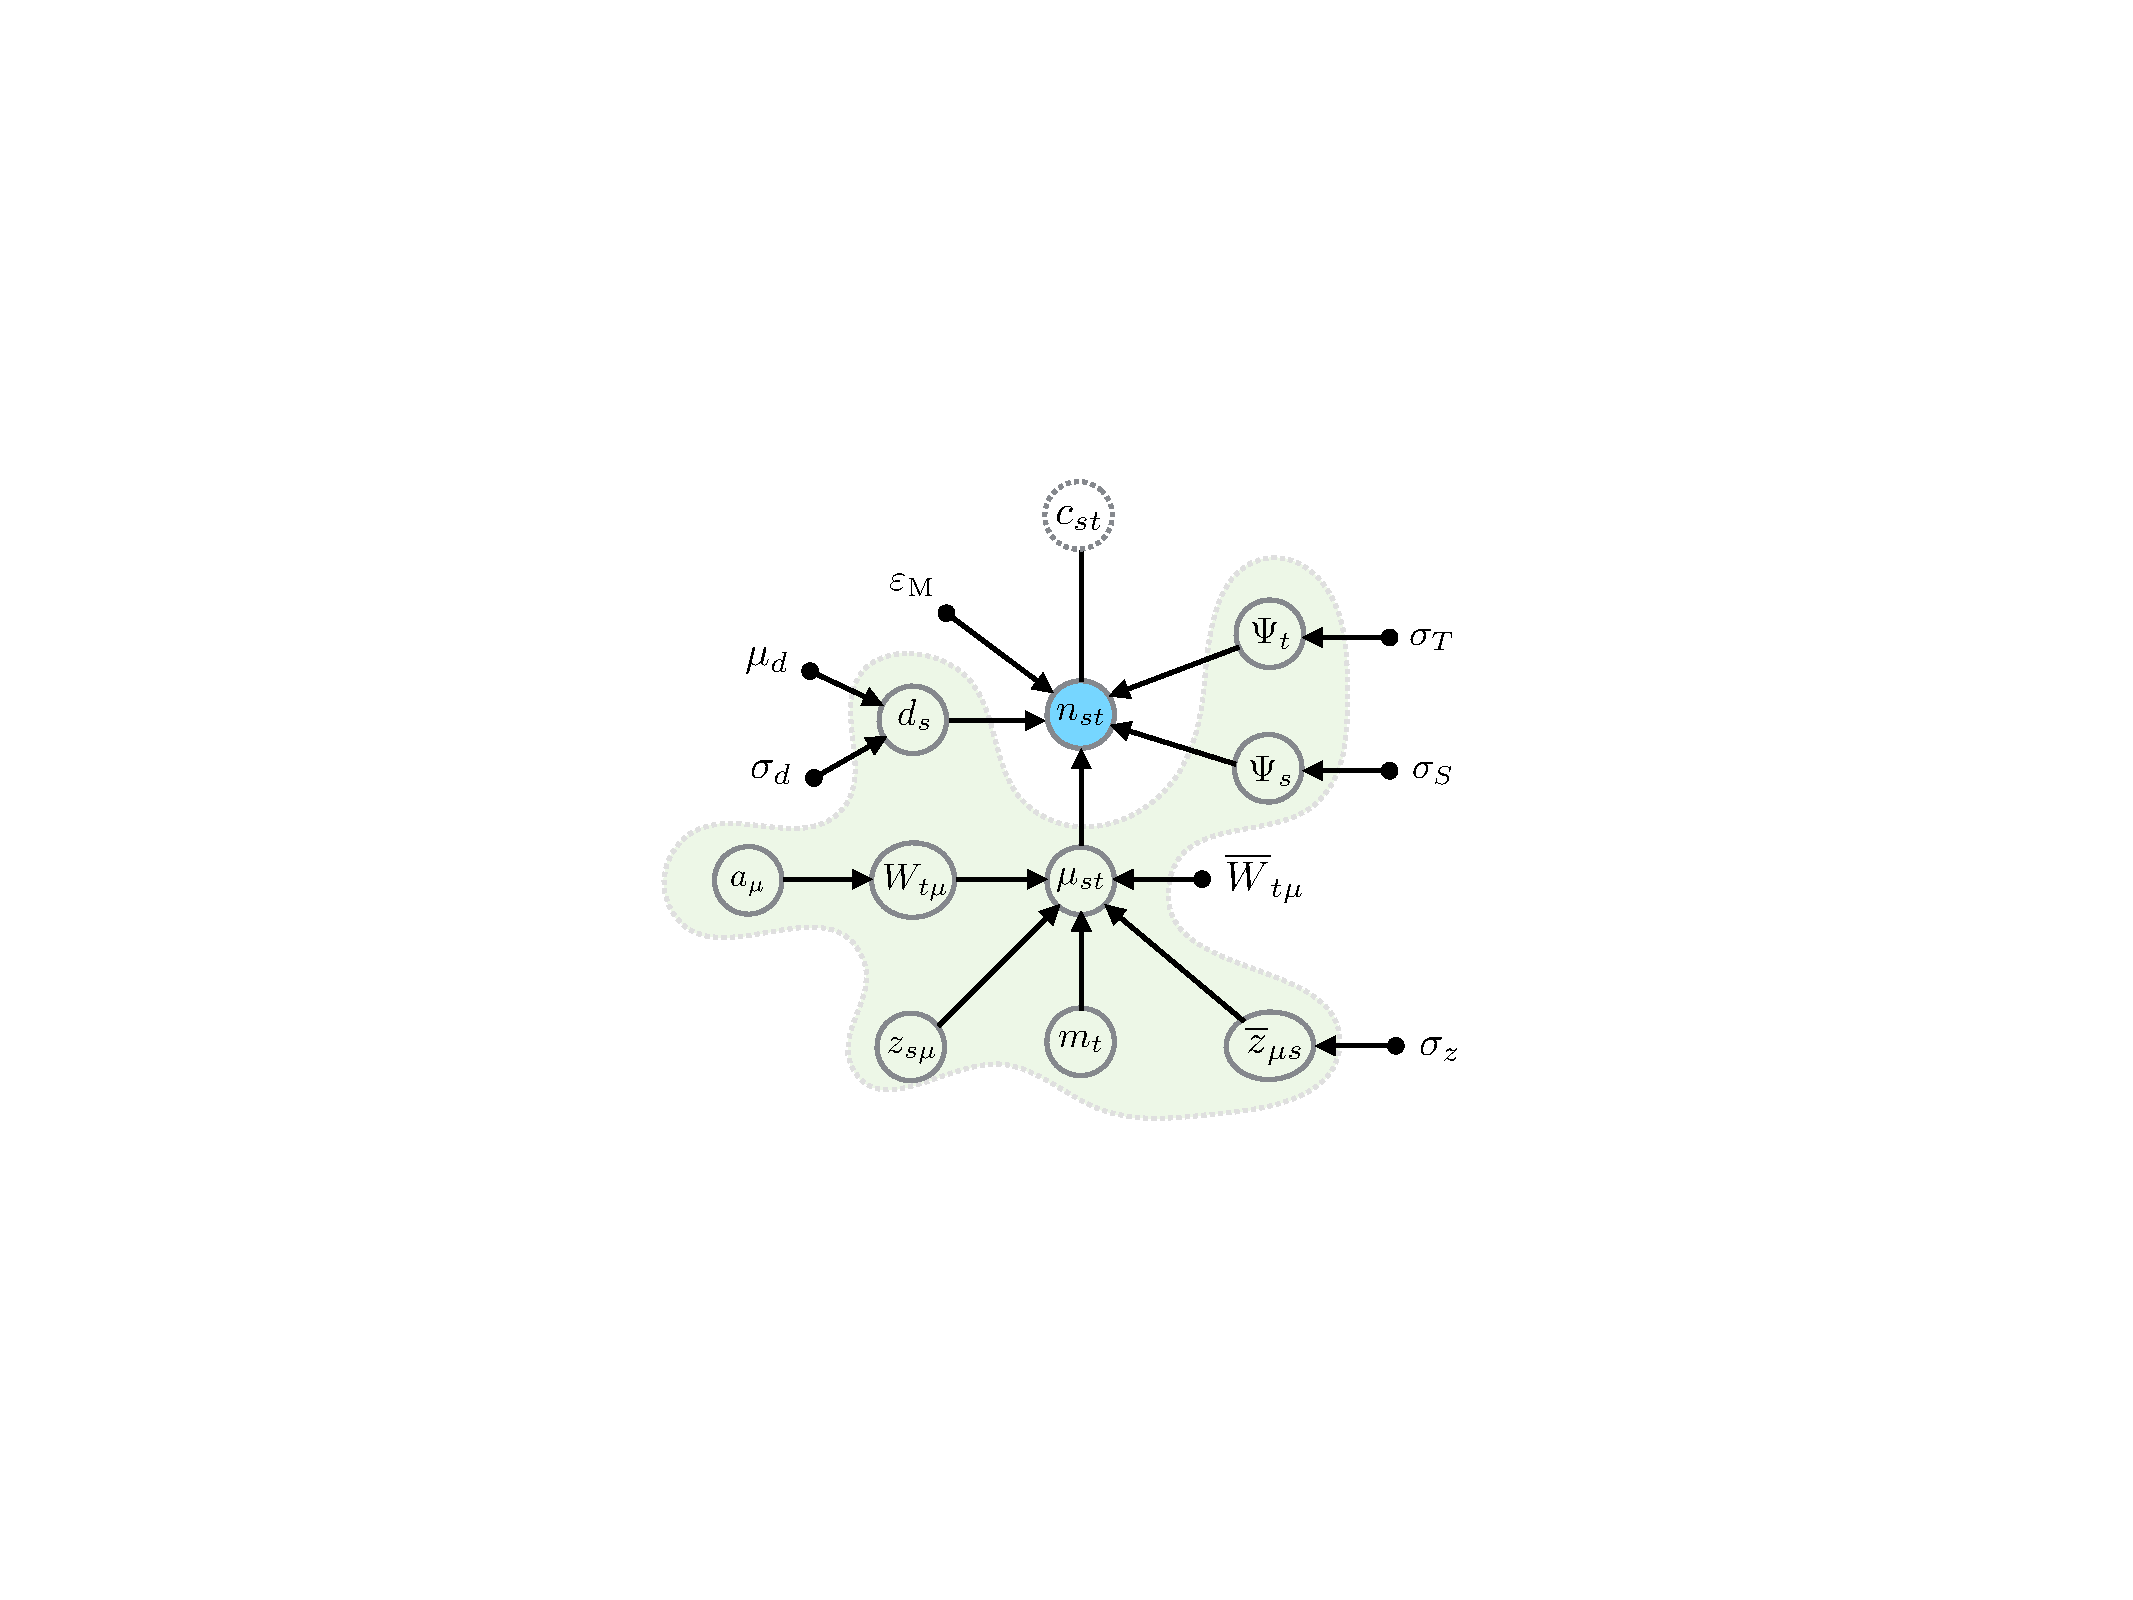
\includegraphics[width=\columnwidth*3/4]{figures/germline-cnv-caller-model/denoising_component.pdf}
\caption{The read-depth model of GATK gCNV.}
\label{fig:denoising_component}
\end{figure}

\noindent{\em\bf Modeling genomic regions and copy-numbers ---}
\begin{figure}
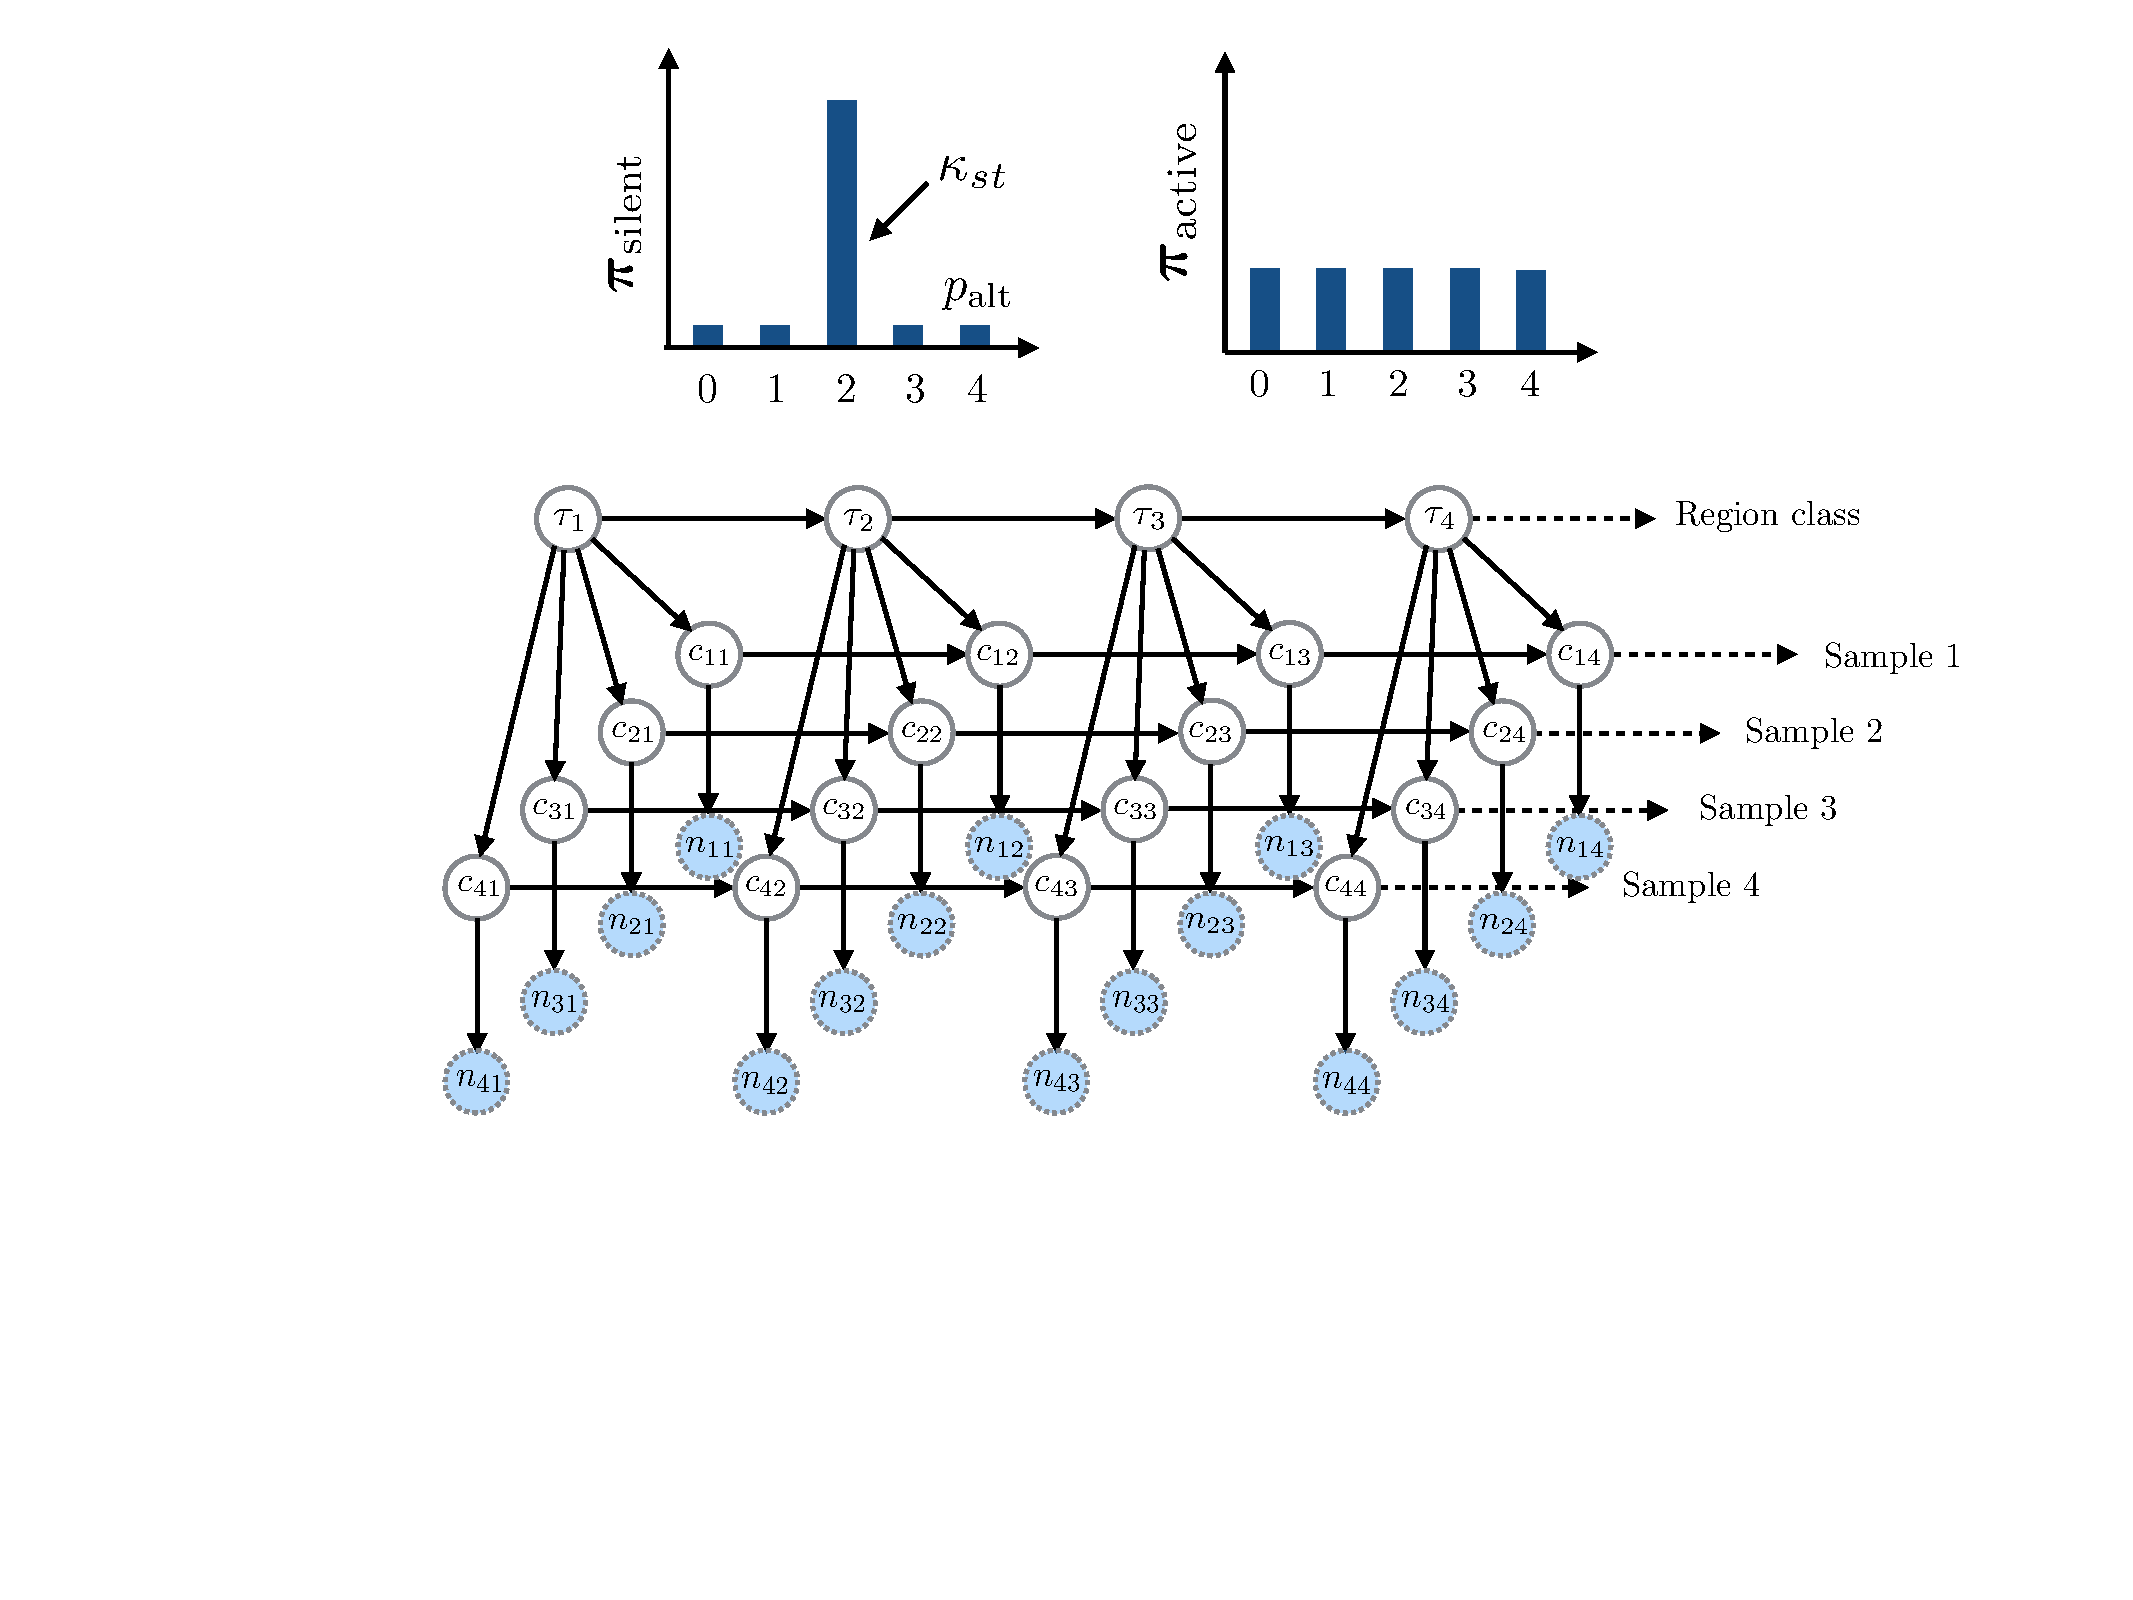
\includegraphics[width=\columnwidth]{figures/germline-cnv-caller-model/hhmm.pdf}
\caption{(top) Copy-number priors for silent and active region classes. (bottom) The hierarchical HMM of region class states and sample-specific copy-number states.}
\label{fig:hhmm}
\end{figure}
Certain genomic regions are biologically more prone to CNV events. We introduce a per-region two-state categorical random variable $\tau_t \in \{\mathrm{silent}, \mathrm{active}\}$ to model such global regional differences. The correlation between genomically close region classes is modeled with an HMM with exponentially decaying transition probabilities:
\begin{multline}
p(\tau_t \rightarrow \tau_{t+1}) = \exp(-\Delta_{t, t+1}/d_\tau) \, \delta(\tau_t, \tau_{t+1}) \\+ [1 - \exp(-\Delta_{t, t+1}/d_\tau)]\,p(\tau_{t+1}),
\end{multline}
where $p(\tau_{t})$ the prior region class probability, $\Delta_{t, t+1}$ is the genomic distance between region $t$ and $t+1$, and $d_\tau$ is the typical size of regions with similar CNV activity rates.

Sample-specific copy-numbers are modeled similarly, with one Markov chain per sample; however, priors and transition probabilities are conditioned on the region class $\tau_t$. We set a {\em baseline} copy-number state matrix for each sample $\kappa_{st}$ in a preliminary modeling step that estimates chromosome-level copy numbers. That is, $\kappa_{st}$ denotes the copy-number state in the absence of any CNV event. We use a prior copy-number probability that strongly prefers the baseline state $\kappa_{st}$ in regions where $\tau_t = \mathrm{silent}$ and we use a flat prior where $\tau_t = \mathrm{active}$. The copy-number transition matrix is an exponentially decaying process as before, but with a different decay length $d_\mathrm{CNV}$ and per-region priors. The dependency relations of the resulting hierarchical HMM are shown graphically in Fig.~\ref{fig:hhmm}.\\
% The complete model is obtained by attaching the denoising module to emission vertices of the HHMM and is shown in Fig.~\ref{fig:full_model}.

% \begin{figure}
% 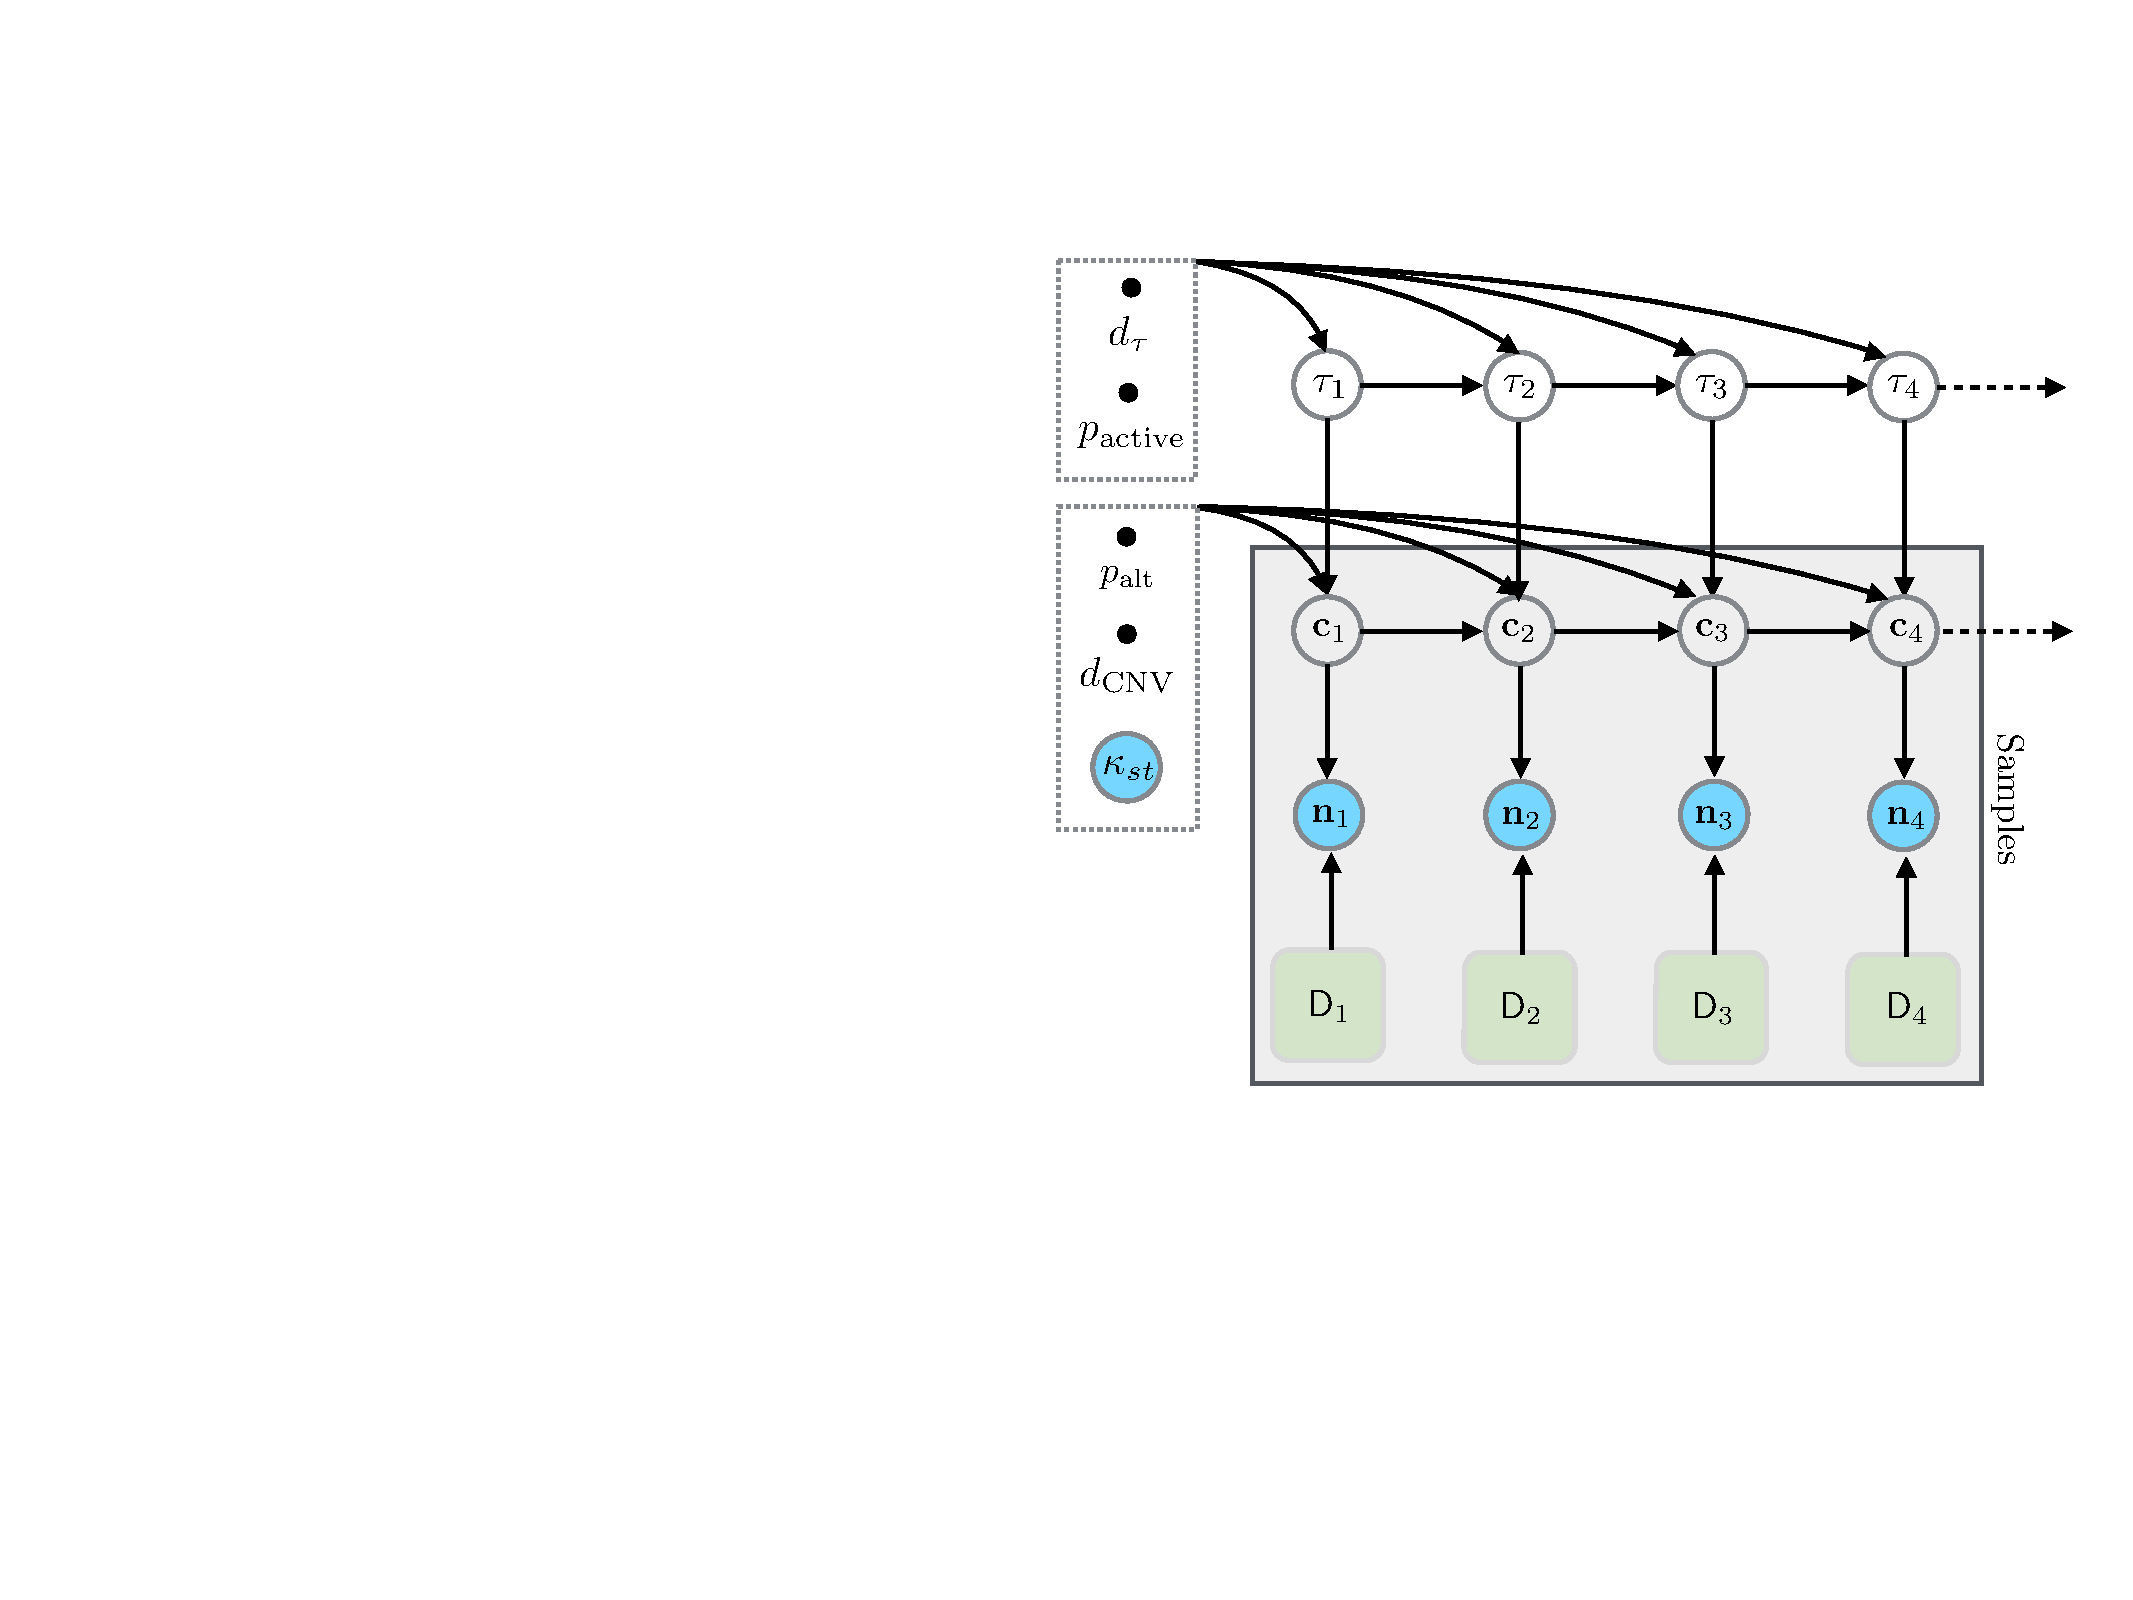
\includegraphics[width=\columnwidth]{figures/germline-cnv-caller-model/full_model.pdf}
% \caption{The complete GATK gCNV graphical model. The $\mathsf{D}_t$ boxes correspond to the denoising components shown in Fig.~\ref{fig:denoising_component}. The HHMM previously shown in Fig.~\ref{fig:hhmm} appears in a schematic form.}
% \label{fig:full_model}
% \end{figure}

\noindent{\em\bf Hybrid ADVI framework ---} The GATK gCNV model contains both continuous and discrete latent random variables (RVs). In order to leverage PPLs and automatic variational inference, we assume a factorized posterior of the form $p(\mathsf{C}, \mathsf{D} | n_{st}) \approx~q(\mathsf{C})\, q(\mathsf{D})$, where $\mathsf{C} = \{m_t, W_{t\mu}, \ldots\}$ and $\mathsf{D} = \{c_{st}, \tau_t\}$ denote the set of continuous and discrete latent RVs, respectively. Subsequently, the full evidence lower bound (ELBO) admits a natural partitioning $\mathsf{ELBO} = \mathbb{E}_{\mathsf{C} \sim q(\mathsf{C})}[\mathsf{ELBO}|\mathsf{C}] + \mathbb{E}_{\mathsf{D} \sim q(\mathsf{D})}[\mathsf{ELBO}|\mathsf{D}]$. Given $q(\mathsf{D})$ and a variational ansatz for $q(\mathsf{C})$, the ELBO can be increased by performing gradient descent steps on the parameters of $q(\mathsf{C})$. Likewise, given $q(\mathsf{C})$, one can gather sufficient statistics via posterior sampling to apply Bayesian updates on $q(\mathsf{D})$; see below. We refer to this scheme as {\em Hybrid ADVI}.\\

\noindent{\bf Continuous sector: {\em ADVI} ---} We implement inference for the continuous RVs using the PyMC3 PPL~\cite{salvatier_probabilistic_2016}. We assume a fully factorized Gaussian variational posterior for $q(\mathsf{C})$, which is updated using ADVI \cite{Kucukelbir:2017:ADV:3122009.3122023}. Once partial convergence is achieved, we move on to the discrete sector. It can be shown that a sufficient statistic for a Bayesian update of $q(\mathsf{D})$ is the $q(\mathsf{C})$-averaged {\em log emission probability}, $\mathbb{E}_{\mathsf{C} \sim q(\mathsf{C})}[\log p(n_{st} | c_{st}, \mathsf{C})]$, which we obtain via sampling.\\

\noindent{\bf Discrete sector: {\em variational message passing} ---} Performing an exact Bayesian update of $q(\mathsf{D})$ is feasible via message passing; however, this has an exponential complexity in the number of per-sample Markov chains ($S$). Assuming $\mathsf{S} \gg 1$, we expect the posterior $q(\tau_t)$ to become sharp, resulting in an effective decoupling of $\tau_t$ (parent chain) and $c_{st}$ (child chains). Therefore, we assume an ansatz $q(\mathsf{D}) \approx q(\tau_t) \prod_{s=1}^S q_s(c_{st})$, neglecting correlations between $\tau_t$ and $c_{st}$ {\em and} between different child chains, but retaining genomic correlations along each chain. This allows us to update $q(\tau_t)$ and $q_s(c_{st})$ using the standard forward-backward algorithm, although we must use mean-field effective prior and transition probabilities that need to be self-consistently determined.  For brevity, we omit the derivation of the iterative scheme, but note that self-consistency is achieved quickly after 2-3 rounds of forward-backward updates with relaxation.  The complexity of our variational treatment of this HHMM is $\mathcal{O}(S T C^2)$, where $C$ is the number of allowed integer copy-number states; crucially, this is linear in $S$.\\

\noindent{\em\bf Marginalized warm-up and deterministic annealing ---} The complete inference scheme involves interleaving updates of $q(\mathsf{C})$ and $q(\mathsf{D})$. In practice, we found that the non-convexity of ELBO yielded spurious local minima with poor initialization. To alleviate this issue, we utilize two techniques: (1) We initialize $q(\mathsf{C})$ and $q(\mathsf{D})$ by {\em approximately} marginalizing all discrete RVs, and obtain the first estimate of $q(\mathsf{C})$ from the marginalized model. (2) In the spirit of the deterministic annealing expectation-maximization (DA-EM) algorithm \cite{ueda_deterministic_1998}, we apply entropic regularization to both the continuous and the discrete RVs. In brief, we initially encourage high-entropy variational posteriors by replacing the standard ELBO with $\mathsf{ELBO}(\beta) = \mathbb{E}_{\mathbf{z} \sim q(\mathbf{z})}[\log p(\mathbf{x}, \mathbf{z}) - \beta q(\mathbf{z})]$, where $\beta \geq 1$ is the inverse temperature and is slowly annealed during learning. A similar recipe applies to the variational message passing, where all prior, transition, and emission probabilities are scaled by $\beta^{-1}$ in log space and renormalized. Our PyMC3 implementation of DA-ADVI is provided with GATK \cite{mckenna_genome_2010}.

\section{Benchmarking}\label{sec:bench}
\begin{figure}
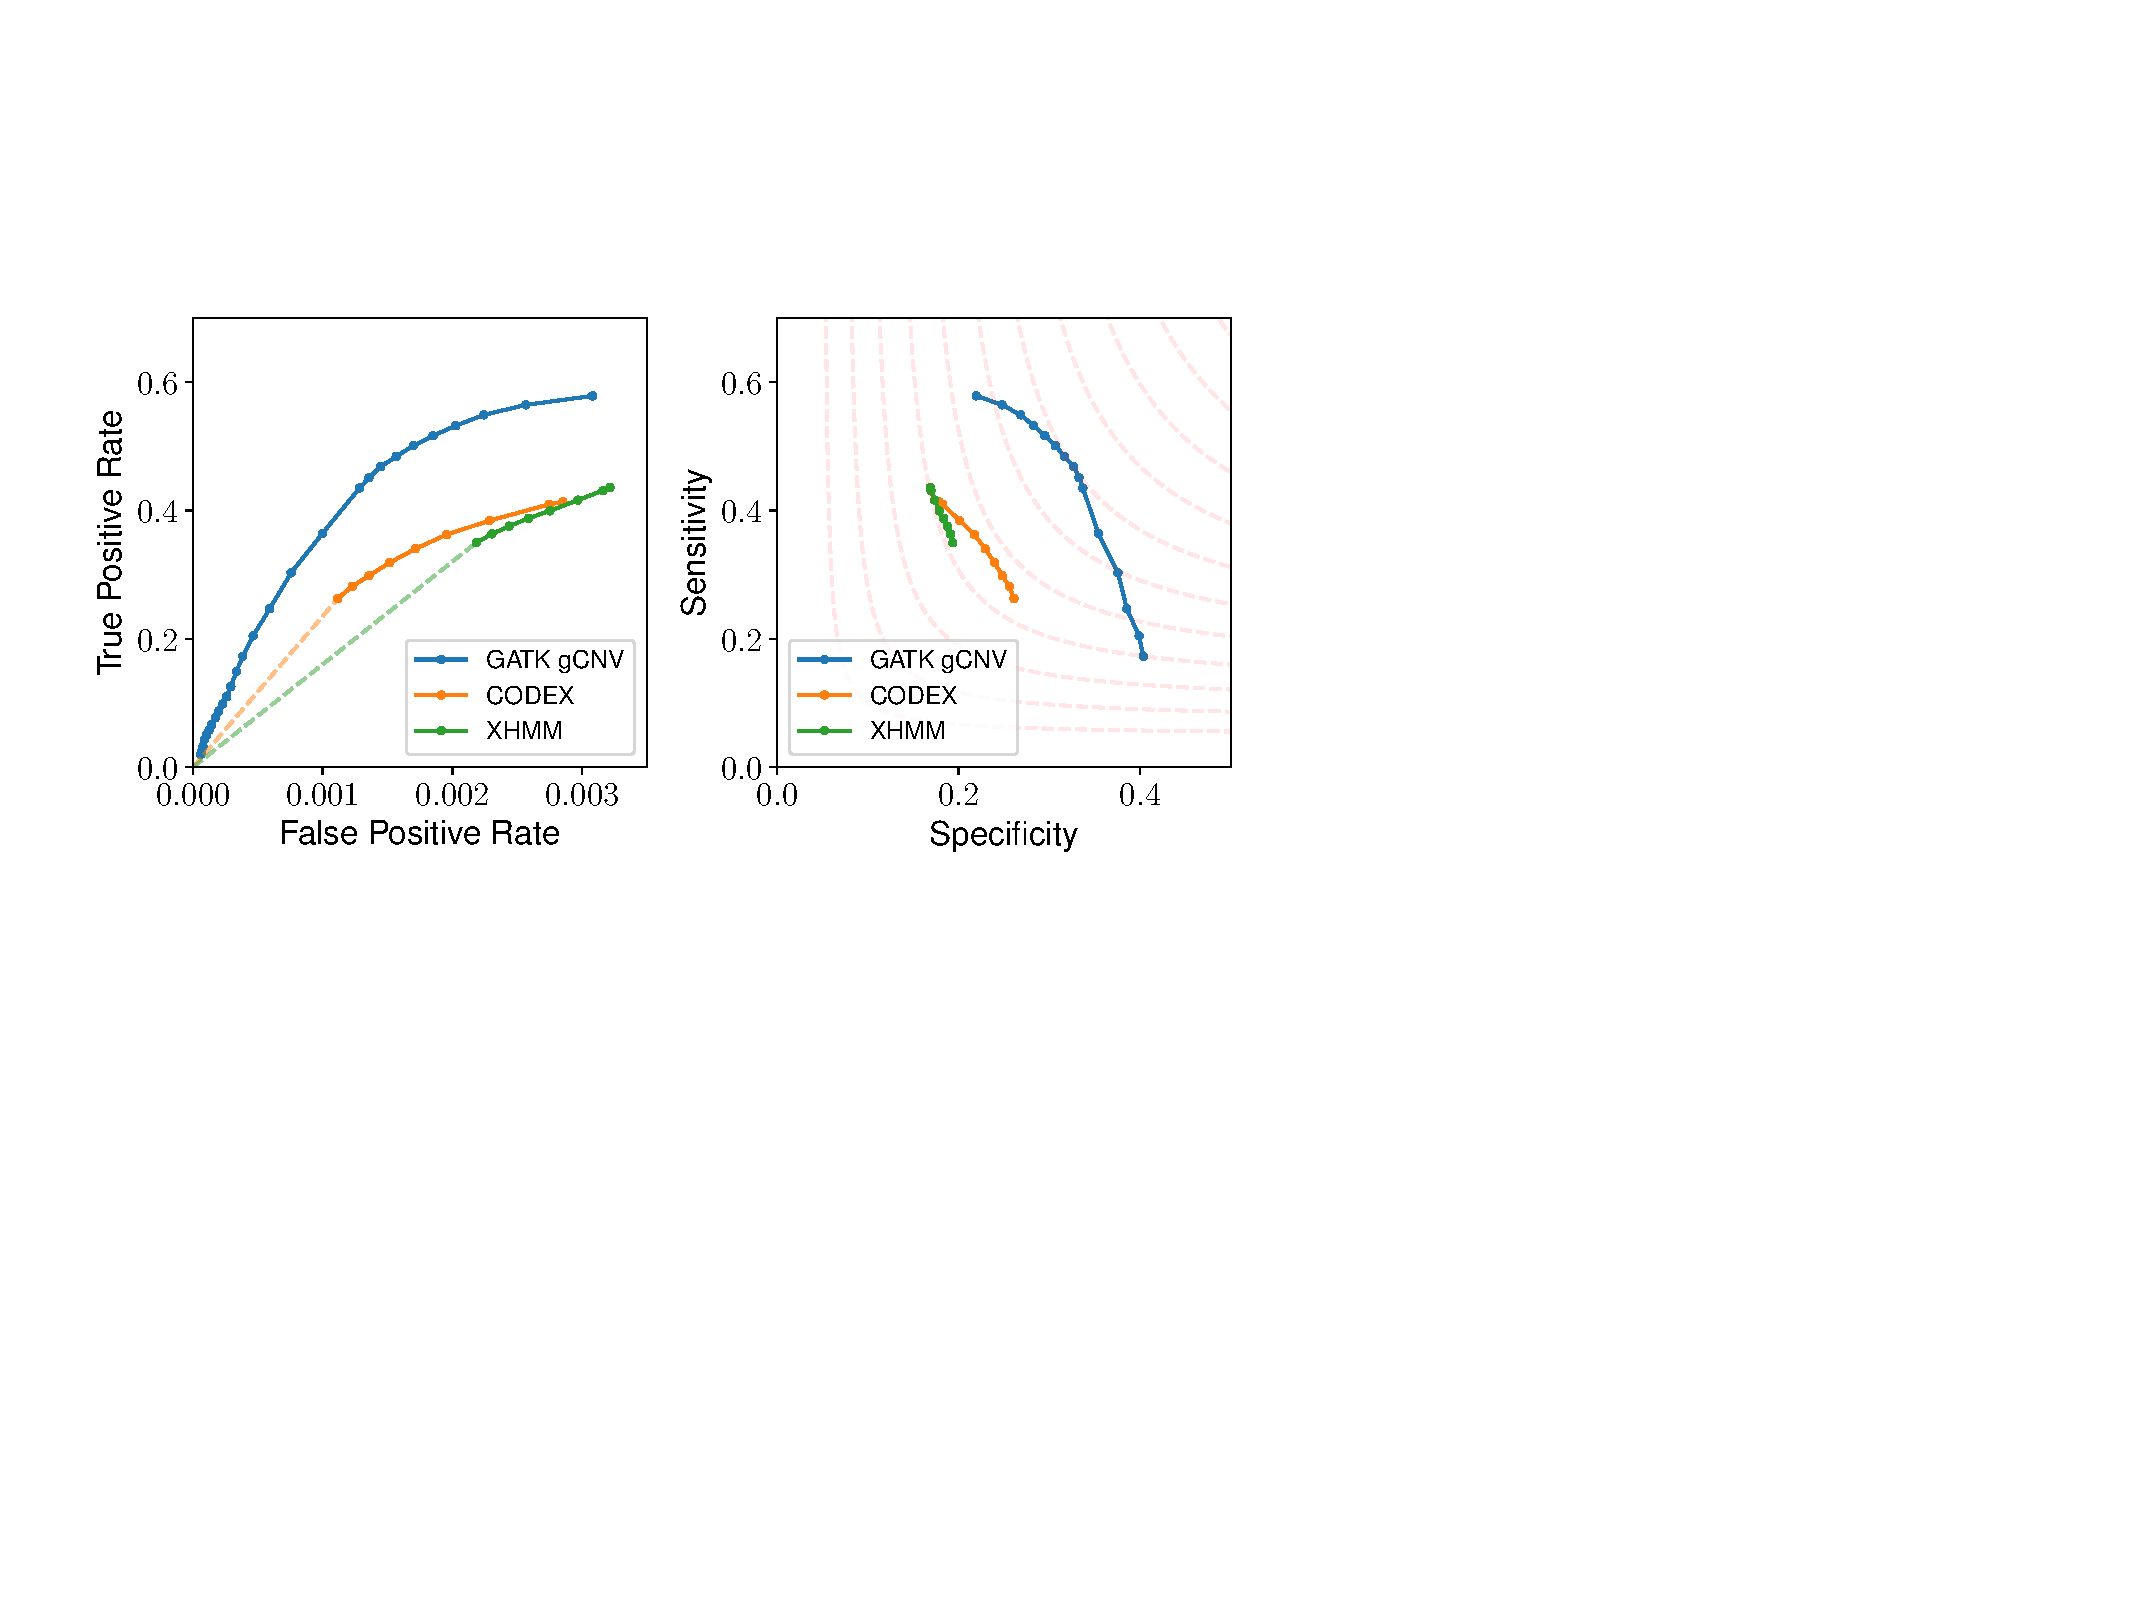
\includegraphics[width=\columnwidth]{figures/germline-cnv-caller-model/benchmark.pdf}
\caption{The performance of GATK gCNV, XHMM \cite{fromer_discovery_2012}, and CODEX \cite{jiang_codex:_2015} in detecting CNV events from WES data against a matched WGS callset obtained using Genome STRiP \cite{handsaker_large_2015}.  Performance metrics are reported per WES target.}  
\label{fig:benchmark}
\end{figure}
Finally, we benchmark GATK gCNV using a cohort of whole-exome sequencing (WES) blood-normal samples. We use a manually validated and FDR-controlled callset obtained from matched whole-genome sequencing (WGS) samples using Genome STRiP~\cite{handsaker_large_2015} as the truth callset. To compare, we also include the CNV calls obtained using two popular CNV calling tools, XHMM \cite{fromer_discovery_2012} and CODEX \cite{jiang_codex:_2015}, in the benchmark. The results are shown in Fig.~\ref{sec:bench}. We find that GATK gCNV yields nearly $20\%$ higher sensitivity and $50\%$ higher specificity over all CNV events compared to the other methods.  Although not presented here, benchmarks that stratify by truth variant frequency also show that GATK gCNV performs favorably on common CNV events. More extensive benchmarking results demonstrate even further improvement, primarily resulting from GATK gCNV hyperparmeter optimization using additional WGS truth callsets, and will be presented elsewhere.

\bibliography{germline-cnv-caller-model}

\end{document}
